\documentclass[12pt]{article}


\usepackage{wrapfig}
\usepackage{float}
\usepackage{graphicx}
\usepackage[margin=1in]{geometry} 
\usepackage{amsmath,amsthm,amssymb}
\usepackage[vlined,linesnumbered,ruled,resetcount]{algorithm2e}

\DeclareMathOperator*{\argmax}{arg\,max}
\DeclareMathOperator*{\val}{val}

\renewcommand\thesubsection{(\alph{subsection})}

% \usepackage[noend]{algpseudocode}
% \usepackage{algorithm}
% \usepackage{algorithmicx}

\newcommand{\N}{\mathbb{N}}
\newcommand{\Z}{\mathbb{Z}}

\newtheorem{definition}{Definition}
\newtheorem{lemma}{Lemma}
\newtheorem{theorem}{Theorem}
\newtheorem{conjecture}{Conjecture}

\begin{document}

% \renewcommand{\qedsymbol}{\filledbox}
 
\title{You can't handle the lie: \\
  Catching lying actors in the BGP protocol }
\author{Clay Thomas, Gavriel Hirsch\\
claytont@princeton.edu, gbhirsch@cs.princeton.edu }
\maketitle

\begin{abstract}
  In many BGP networks, nodes can get their preferred path
  by advertising a certain path, but forwarding traffic along another.
  However, in many of the example networks from the literature,
  other nodes can collectively detect these lies
  by comparing the route that is advertised (known by the node
  the manipulator lies to)
  to the route actually taken
  (known by the node the manipulator actually forwards traffic to).
  We want to study the conditions under which nodes
  can lie without being detected,
  as well as the economic incentives of other nodes to collaboratively
  check each other (such as providers helping customers detect liars).
\end{abstract}

\section{In the \cite{RoutingGames} model, you can always catch a liar}

  \begin{conjecture}
    Suppose No Dispute Wheel holds, but route verification does not, and
    assume that the network is connected.
    Suppose that (assuming other nodes play truthfully)
    a node $m$ can achieve a better path to $d$ by announcing
    a route that does not exist to a node $v$.
    Let $m$'s next hop in the manipulated routing tree be denoted $r$.
    Then there exists a path in the network, not containing $m$,
    between $v$ and $r$.
  \end{conjecture}
  % \begin{proof}
  %   For the sake of contradiction, assume that all paths between $r$
  %   and $v$ include $m$.
  %   One of $r$ or $v$ is on the ``same side of $m$'' as the destination
  %   node $d$. But the routing on different sides of $m$ cannot directly effect
  %   each other, or at least that would be really weird.

  %   It would be nice if I could make this precise before Friday.

  %   % We know that $m$ lies to node $v$ in order to
  %   % get $r$ to select a path it likes better.
  %   % Because $v$ (and all other nodes) act honestly by best-reply dynamics,
  %   % we know $v$ must have changed its route after hearing $m$'s lie.
  %   % This, in turn, broke $r$'s original route to $d$.
  %   % Thus, $v$ must lie along $r$'s original path to $d$,
  %   % so $v$ and $r$ are connected in the network.
  %   % Furthermore, 

  %   % Let $T$ denote the (unique) routing tree resulting from
  %   % all players honestly following BGP.
  %   % For any node $x$ in the graph, let $T_x$ denote the full path
  %   % from $x$ to $d$ in $T$.
  %   % Let $M$ denote the routing tree resulting from $m$'s lie,
  %   % and define $M_x$ similarly to $T_x$.
  %   % We know that $T_r \ne M_r$, because $v_m(T_r) < v_m(M_r)$.
  %   % Let $p$ be the node along path $T_r$ such that
  %   % $T_p\ne M_p$ and $p$ is as close to $d$ as possible.
  %   % Then $p$ must have a different next-hop in $T$ than in $M$
  %   % (if the next-hop in $T$ and $M$ were the same, then the next-hop $p'$
  %   % of $p$ would satisfy $T_{p'}\ne M_{p'}$, yet be closer to $d$ along $T_r$).
  % \end{proof}

  This means that, if all nodes other than $m$ are fully collaborative and
  honest, the nodes will be able to detect $m$'s lie
  by communicating along the links that already exist in the network.

  \subsection{In the \cite{Attraction} model, you can't}
    Consider Bowtie (figure~\ref{fig:Bowtie}),
    an example taken directly from \cite{Attraction}.
    In this case, node $m$ needs to lie to nodes $c$ and $n$,
    but actually forward traffic to node $d$.
    The only nodes between $d$ and $c$ (or $n$) pass through node $m$.
    Thus, the honest nodes cannot catch $m$ in its lie solely using 
    the communication channels provided by the network itself.

    \begin{figure}[h]
      \centering
      \caption{Bowtie}\label{fig:Bowtie}
      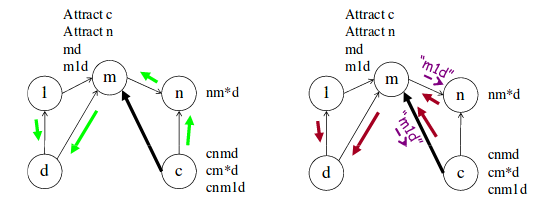
\includegraphics[width=0.75\textwidth]{Bowtie}
    \end{figure}

    One objection may be that real-life networks are much more highly
    connected than the small counterexamples presented in these papers.
    However, we believe that very small sets of nodes surrounding
    the adversary $m$ can reasonably model the set of nodes
    that actually \emph{care} enough to try and catch $m$ lying.
    Thus, it makes sense to ask if small subnetworks can catch $m$
    communicating only along links among themselves.


\section{But will you?}
  Figure~\ref{fig:Nonexistent} shows an example network
  (taken directly from \cite{RoutingGames}
  but rendered in the style of \cite{Attraction})
  where $m$ has an incentive to advertise a path that does not exist.
  We regard this network as the canonical example of Conjecture 1.
  Indeed, node $1$ can inform node $2$ that it is receiving traffic
  from $m$, so $2$ will know that $m$ is lying about its path.
  \begin{figure}[h]
    \centering
    \caption{Nonexistent}\label{fig:Nonexistent}
    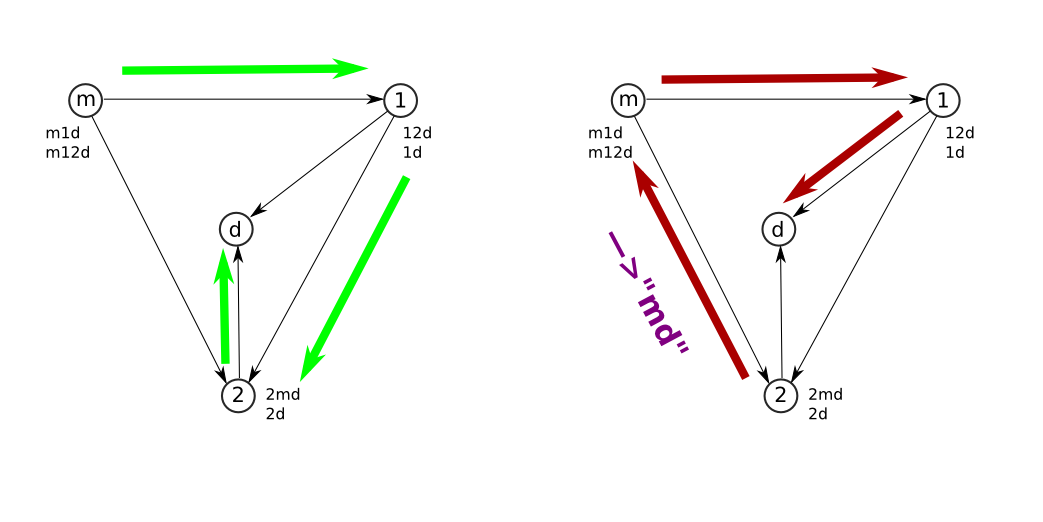
\includegraphics[width=0.75\textwidth]{NonexistentBetter}
  \end{figure}

  This example is a Gao-Rexford network, where customer-provider
  relationships are denoted by arrows pointing from customers to providers.
  Note that node $2$ must be a provider of node $1$ for this example
  (otherwise, $2$ would not export its route to $d$ to $1$).
  In general, customers do not provide services for their providers,
  so it may not make sense for node $1$ to help node $2$ catch $m$'s lie.
  Thus, it is not reasonable to assume that $1$ will want to help
  $2$ detect the lies of $m$, because $1$ does not perform services
  for its provider $2$.
  On the other hand, if $1$ does inform $2$ of the lie, and $2$ resumes
  using its old route, $1$ actually gets a path that it prefers.

  Thus, we regard the competing incentives of
\begin{itemize}
\item getting good paths
\item economic obligations of customer-provider relationships
\item costs of maintaining and communicating lie-detecting information
\end{itemize}
to be an interesting avenue of research

  \section{Project Components}
  We plan to first analyze which situations can result in a node having an incentive to lie and other nodes having incentives to not expose that lie to each other. In addition we will design a new protocol and consider corresponding business relationships in which nodes can both send messages about their paths, and separately share other information that can be used to expose others' lies. We will also analyze situations under this new protocol and see how the analysis differs.



% \section{Notes}
%   Our ideas are related to, but distinct from, the
%   loop verification of \cite{Attraction}.
%   Loop verification required only a very limited form of coordination,
%   where we need nodes to ``just happen'' to snoop and report on each
%   other in just the right way.

\bibliography{proj}{}
\bibliographystyle{alpha}

\end{document}
